\documentclass[12pt,a4paper]{article}
\usepackage{rmpackages}
\usepackage{rmtemplaterapport}

\bibliographystyle{custom-bib/thesis}
\usepackage{bibentry}
\usepackage{pdfpages}


\title{L'expérience de Benjamin Franklin... Et Rayleigh, Pockels, Devaux, et Langmuir}
\author{Rémi Metzdorff}
\date{\today}

\begin{document}

\maketitle

\tableofcontents
\newpage

\section*{Introduction}
\addcontentsline{toc}{section}{Introduction}

Vers la fin du XVIII\textsuperscript{ème} siècle, Benjamin Franklin reverse une petite cuillère d'huile dans un étang près de Londre.
Il remarque que la tache d'huile s'étend rapidement à la surface jusqu'à recouvrir une bonne partie du plan d'eau.
En divisant le volume d'huile renversé par la surface recouverte, on trouve l'épaisseur de la tache d'huile qui s'avère être de l'ordre du nanomètre, c'est à dire la taille d'une molécule d'huile.
Mais ce n'est pas Franklin qui eu l'idée de ce calcul
Lui avait d'autres préoccupations à son époque.

L'expérience est belle : en mesurant deux quantités réellement macroscopiques, on accède à la taille caractéristique d'un des plus petits constituants de la matière.
Il y a quelques années, elle était couramment reproduite à petite échelle au lycée et il existe de nombreuses ressources et activités sur le sujet.
Par exemple, on peut trouver plusieurs articles du bulletin de l'union des physiciens (BUP) \cite{Carron1992, Schwob2000, Bacciochini2002, Serra2002} sur ce thème.
L'expérience est toutefois plus subtile qu'il n'y parait peut-être, ce qui explique à la fois son interprétation tardive et les difficultés rencontrées parfois pour la reproduire.

Le billet de blog de David Louapre~\cite{Louapre2012} constitue une bonne introduction au sujet.
À sa lecture on se rend bien compte qu'attribuer tout le mérite de cette expérience à Benjamin Franklin est un peu exagéré.
C'est grâce à un article du bulletin de l'union des physiciens~\cite{Bolmont2001} que j'ai pu orienter mes recherches sur les différents auteurs ayant contribué à la compréhension de cette expérience et cibler les articles utiles.

\section{L'expérience historique et son interprétation}

L'expérience est relatée par Benjamin Franklin lui même dans une lettre adressée à William Brownrigg\cite{Franklin1773a} :
\begin{itemize}
\item[]
\textit{ \og
At length being at Clapham where there is, on the common, a large pond, which I observed to be one day very rough with the wind, I fetched out a cruet of oil, and dropped a little of it on the water.
I saw it spread itself with surprising swiftness upon the surface ;
[...] the oil, though not more than a tea spoonful, produced an instant calm over a space several yards square, which spread amazingly and extended itself gradually till it reached the lee side, making all that quarter of the pond, perhaps half an acre, as smooth as a looking-glass.
\fg{} }.
\end{itemize}
Le reste de la lettre montre que la préoccupation de Franklin n'est pas la mesure de la taille des molécules d'huile.
Lui s'intéresse plutôt au calme produit par l'huile sur une surface d'eau agitée par le vent~\cite{Mertens2006}.

Il faut attendre plus d'un siècle pour que Rayleigh reprenne le principe de cette expérience et en déduise l'épaisseur de la couche d'huile~\cite{Rayleigh1890a}.
Pour cette article, il mesure la masse d'huile d'olive nécessaire pour stopper le mouvement de copeaux de camphre à la surface d'une bassine d'eau.
\footnote{À cette époque, il semble que le camphre soit couramment utilisé comme indicateur de la tension de surface de l'eau.
Dans un autre article~\cite{Rayleigh1892}, } 
D'après 

\cite{Rayleigh1890a}, Measurements of the amount of oil necessary in order to check the motions of camphor upon water.
Il mesure la masse d'huile nécessaire pour arrêter le mouvement de camphre sur un grand bac d'eau et en déduit l'épaisseur du film correspondant.

\cite{Pockels1891}, Surface Tension.
Diverses expériences sur la tension de surface dans une lettre envoyée à Rayleigh.
Surface normale : la tension de surface ne dépend pas de l'aire de la surface d'eau dans son dispositif.
Surface anormale : a tension de surface dépend fortement de l'aire.
Courant de solution.
Solubilité de surface très élevée.

\cite{Rayleigh1892} : Experiments upon surface-films.
On comprend pourquoi ils utilisent le camphre comme indicateur de la tension de surface.
Il est dit que lorsque le camphre ne bouge plus, la tension de surface est en dessous de 0{,}72 fois celle de l'eau. 

\cite{Pockels1894} : On the Spreading of Oil upon Water.
Elle décrit très bien ce qu'il se passe si on ajoute de l'huile sur une surface saturée, même si cela semble déjà bien connu (\cite{Rayleigh1892}).

\cite{Rayleigh1899} : Investigations in capillarity.
Reproduction des expériences de Pockels (\cite{Pockels1891}), mesure de la tension de surface d'une eau contaminé avec de l'huile avec un tensiomètre à plaque de Wilhelmy.
Discussion sur l'état normal et l'état anormal de la surface.
Évoque la nécessité d'utiliser la notion de molécule pour expliquer la transition.
Discrétisation des valeurs de tension superficielle suivant le nombre de couches monomoléculaires.
Il suppose une couche monomoléculaire et en déduit le diamètre d'une molécule d'huile : \unit{1}{nm}.

\cite{Devaux1904} : Comparaison de l'épaisseur critique des lames très minces avec le diamètre théorique des molécules.
Tout est dans le titre, il semblerai qu'il soit le premier à comparer la hauteur du film avec la taille théorique des molécules.
Celle-ci est fournie grâce aux travaux de Nernst qui se base sur des considérations thermodynamiques (théorie cinétique des gaz : libre parcours moyen des molécules, section efficace) pour calculer les grandeurs moléculaires.

1913 : Marcelin, Epaisseur des couches très minces à la surface de l'eau, Diplôme d'études sup., Paris (1913), Ann. de Phys. (1913). Texte non trouvé

\cite{Langmuir1917} : The constitution and fundamental properties of solids and liquids. II. Liquids.
En plus d'une revue très claire des apports de Rayleigh, Pockels, Devaux et Marcelin, il évoque les raisons qui poussent le film d'huile à s'étendre et discute l'orientation des molécules d'huile à la surface de l'eau.
Ses considération théoriques sur les propriétés hydrophiles du groupement carboxyle (et de la double liaison) et hydrophobe des chaines carbonées sont suivies d'expériences permettant de déterminer à la fois la longueur des molécules d'huiles (l'épaisseur du film d'huile) et leur diamètre (en estimant la surface occupée par chaque molécule connaissant le nombre de molécule déposé).
Il tord aussi le coup aux hypothèses de film bi-moléculaire proposés par Rayleigh et Marcelin en invoquant la notamment souplesse des chaines carbonées.

\cite{BiolinScientific2011} : Fabricating Highly Organized Nanoparticle Thin Films.
Aujourd'hui, le procédé de déposition Langmuir-Blodgett permet d'obtenir des film mono ou multicouche de composés variés.

\section{Analyse de l'expérience en seconde}

\subsection{Dans le programme}

\subsection{L'activité}

\subsubsection{Déroulement de la séance}

\begin{itemize}
\item[0h00]
Début de la séance.

Accueil des élèves, désinfection des mains, placement libre par binôme, \og Bonjour à tous, asseyez-vous. \fg{}, Appel.

\item[0h05]
\og Aujourd'hui, on va essayer de répondre à la question : Quelle est la taille d'une molécule d'huile ? 
\textcolor{red}{(écrit au tableau : Quelle est la taille d'une molécule d'huile ? )}

\og Un compte-rendu chacun,  j'en ramasserai un au hasard par groupe à la fin de la séance. \fg{}

\og Sur le document que je vais vous distribuer, je vous ai mis une aide pour la rédaction du compte-rendu.
Comme les autres fois, la première étape sera d'écrire votre hypothèse et de la justifier.
Commencez bien par ça ! \fg{} 

\og Je vous laisse découvrir le document et démarrer. \fg{}

\textcolor{red}{Préparer la fiche de notation avec le nom des binômes.}

\item[0h20]
Aide collective.

\og Si vous avez du mal à démarrer, puisqu'il est question d'une cuillère à café dans la lettre, commencez par déterminer le volume d'une cuillère à café.
\textcolor{red}{(écrit au tableau : Aide 1 : Déterminer le volume d'une cuillère à café.)}
Vous en avez au bureau. \fg{}
\begin{itemize}
\item Aide : Avec quelle verrerie peut-on mesurer un volume ?

\item Aide : Mesure le volume d'une cac d'huile avec une éprouvette

\item Aide : Une cac fait 5 mL
\end{itemize}

\item[0h50] (indicatif)
Aide pour décoincer ceux qui bloquent après la mesure du volume.

\textcolor{red}{Distribuer ponctuellement schéma et formule du volume d'un cylindre aplati.}

\begin{itemize}
\item Aide : Dans la formule, quelles sont les valeurs connues ?
\item Aide : Mesure l'aire sur le schéma
\item Aide : L'aire de la flaque est \unit{2000}{m\squared}
\end{itemize}

\item[1h05]
\og Il vous reste 20 min \fg{}

\begin{itemize}
\item Aide : Ça vous semble normal de trouver un chiffre aussi petit ?
\item Aide : Le professeur verse des haricots sur la table
\item Aide : L'huile forme une couche haute comme une seule molécule
\end{itemize}

\item[1h20]
\og Il vous reste 5 min pensez à bien ranger votre table. \fg{} 

Nettoyage

\textcolor{red}{Ramasser les compte-rendus}
 
\item[1h25] Fin de la séance
\end{itemize}

\subsubsection{Matériel}

Le matériel est à disposition des élèves mais pas directement sur leur paillasse :
\begin{itemize}
\item[•] bécher \unit{100}{mL} ;
\item[•] éprouvette graduée \unit{10}{mL} ;
\item[•] balance ;
\item[•] cuillère à café ;
\item[•] entonnoir ;
\item[•] eau ;
\end{itemize}

\subsubsection{Évaluation}

Lors de la séance, l'évaluation est portée sur trois compétences en particulier : \anarai{}, \rea{} et \val{}.\footnote{Puisque l'activité est un problème ouvert, d'autres compétences sont inévitablement mobilisées mais il est possible de les évaluer après la séance sur la base du compte-rendu rédigé par les élèves.
Ce n'est pas sur celles-ci que l'accent est mis pour cette activité.}
La maitrise de ces compétences est graduée selon quatre niveaux identifiables d'après l'aide apportée lors de la séance : A (bien maitrisée), B (maitrisée), C (insuffisamment maitrisée) et D (non maitrisée).
Les observables sont définies dans le tableau~\ref{tab:obs}.

\begin{table}
\center
\begin{tabular}{l|l|c}
\textbf{Compétence} & \textbf{Aptitude} / Observable & \textbf{Niveau} \\
\hline \hline
\anarai 	& \textbf{Élaborer un protocole qui répond à la question} 	& \\
				& L'élève mesure le volume de 10 cac				 						& A+ \\
				& L'élève mesure le volume d'une cac 									& A \\
				& Aide : Avec quelle verrerie peut-on mesurer un volume ?	& B \\
				& Aide : Mesure le volume d'une cac d'huile avec une éprouvette & C \\
				& Aide : Une cac fait 5 mL 															& D \\
\hline
\rea			& \textbf{Faire des observations utiles à l'activité}					& \\
				& L'élève réalise la mesure de l'aire sur le schéma				& A \\
				& Aide : Dans la formule, quelles sont les valeurs connues ? & B \\
				& Aide : Mesure l'aire sur le schéma											& C \\
				& Aide : L'aire de la flaque est \unit{2000}{m\squared}			& D \\
\hline
\val			& \textbf{Avoir un regard critique sur ses résultats}				& \\
				& L'élève fait le lien avec son hypothèse									& A \\
				& Aide : Ça vous semble normal de trouver un chiffre aussi petit ? & B \\
				& Aide : Le professeur verse des haricots sur la table			& C \\
				& Aide : L'huile forme une couche haute comme une seule molécule & D \\
\end{tabular}
\caption{Observables utilisées pour l'évaluation du niveau de maitrise des compétences travaillées lors de la séance.}
\label{tab:obs}
\end{table}

\subsection{Analyse a priori}

Le lien entre l'aspect réellement macroscopique de cette expérience et son interprétation microscopique est sans doute une des principales difficultés de cette activité.
(lien entre espèce chimique et entité chimique présent dans les programmes et abordé en cours)

Si un élève demande à quoi ressemble une molécule d'huile, on peut montrer une molécule d'acide oléique (Fig.~\ref{fig:acide_oleique}).
\footnote{Le composé majoritaire de l'huile d'olive est l'oléine, ou trioléine est un ester dont l'hydrolyse forme l'acide oléique et le glycérol.}
La dimension d'un atome ayant été donnée en cours, on peut s'attendre à ce que l'élève compte les atomes qui composent la \og molécule d'huile \fg{} pour estimer sa taille.
\footnote{Les élèves ont fait une activité similaire en comptant les atomes qui composent le bonhomme du film \href{https://www.youtube.com/watch?v=oSCX78-8-q0}{A boy and his atom} pour estimer sa taille.}
Il se pourrait alors que la forme allongée de la molécule induise un questionnement sur la bonne dimension à prendre en compte.
On peut différer la réponse à cette question en attendant de voir ce que donne les résultats des mesures et calculs et en reparler à la fin du TP : \og D'après vous, comment s'orientent les molécules à la surface de l'eau ? \fg{}.

\begin{figure}
\center
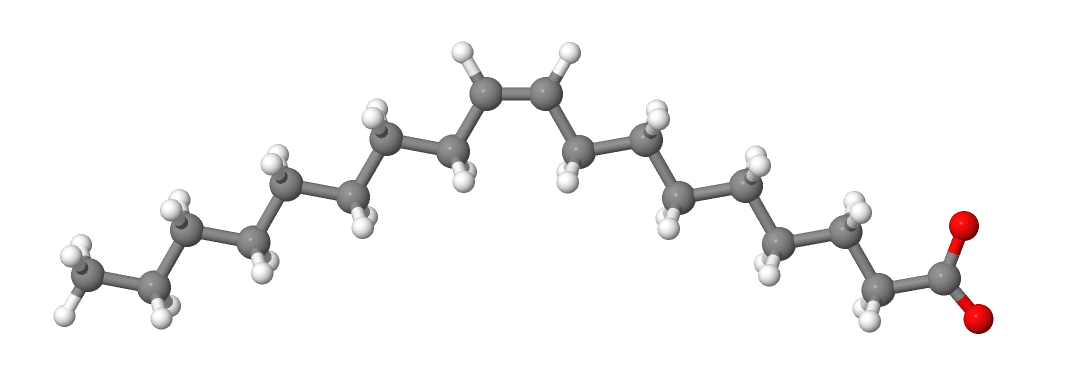
\includegraphics[scale=0.4]{acide_oleique.png}
\caption{Structure d'une molécule d'acide oléique.}
\label{fig:acide_oleique}
\end{figure}

On peut s'attendre à deux méthodes pour la mesure du volume de la cuillère à café : mesure \og directe \fg{} à l'aide d'une éprouvette graduée ou mesure \og indirecte \fg{} à l'aide d'une balance en passant par la masse volumique.  
Dans les deux cas, l'idée de mesurer le volume de plusieurs cuillerées sera valorisé.

On peut s'attendre aussi à ce que l'élève connaisse la valeur du volume d'une cac, ce qui relève plutôt de la compétence \app{} (évaluer quantitativement les grandeurs physiques inconnues et non précisées).
Si la valeur est bonne et que l'élève termine rapidement, on peut l'orienter sur la mesure du volume de la cuillère en l'encourageant à vérifier son hypothèse.

Le schéma du document 2 peut induire un biais : l'étendue de la tache d'huile est simplement repérable par l'absence de vague et pas par sa couleur.
L'épaisseur finale de l'ordre du nanomètre est beaucoup trop faible pour qu'on puisse la repérer optiquement.

\subsection{Analyse a posteriori}

\paragraph{Séance 1 : 2nde1 groupe 2 (30/11)}
\begin{itemize}
\item un groupe part directement sur la mesure de l'aire de la tache d'huile sur le schéma : pour eux, l'aide collective sur la mesure de la contenance de la cuillère d'huile n'a pas de sens.
\item la moitié des élèves pense à utiliser les défis confinés pour déterminer le volume d'une cuillère d'huile.
\item problème avec les unités lors des calculs de volume : ma faute, je l'ai pas précisé dans les calculs.
\item impossible de raisonner avec des considérations de dimension.
\item aucun groupe ne fait le lien entre la question et leur travail bien qu'un groupe soit parvenu à calculer correctement l'épaisseur de la tache.
\item coup de pouce volume du cylindre inadapté : les élèves ne voient pas le rapport entre ce cylindre et l'activité. Pour la suite transformé en \og on a une vue du dessus sur le schéma : dessinez la flaque d'huile en 3D. \fg{}
\item Plusieurs groupes pensent que l'aide du volume permet de calculer... le volume \og Mais on a pas $e$ \fg{}.
Il n'ont pas eu l'idée d'isoler $e$. 
\item les hypothèses sont essentiellement plausibles même si : un groupe semble confondre petites gouttes d'huile et molécule d'huile, un autre propose un volume en mL.
Une molécule c'est la même taille qu'une cellule.
confusion entre atome et molécule.
\end{itemize}


\newpage
\section{Réalisation expérimentale}

Difficile d'avoir une couche mono-moléculaire.
Il faut :
\begin{itemize}
\item soit un grand étang ;
\item soit une très petite quantité d'huile : il faut la dissoudre dans un solvant volatil.
\end{itemize}
Historiquement, c'est le benzène (appelé benzine à l'époque) mais ça va pas trop toxique.
Dans les protocoles plus modernes, on utilise de l'essence de térébenthine mais ça va pas c'est trop peu volatil et toxique.
Il faudrait essayer l'acétate d'éthyle : aussi volatil que le benzène mais beaucoup moins toxique.
 

\begin{table}
\center
\begin{tabular}{l|c|l}
\textbf{Composé} & $P_\mathrm{sat}^{\unit{20}{\celsius}}$ (mbar) & \textbf{Toxicité} \\
\hline \hline
Éther diéthylique & 586 & H224, H302, H336 \\
Cyclohexane & 127 & H225, H304, H315, H336, H410 \\
Benzène & 100 & H225, H304, H315, H319, H340, H350, H372 \\
Acétate d'éthyle & 100 & H225, H319, H336 \\
Éthanol & 58 & H225 \\
Toluène & 29 & H225, H304, H315, H336, H361d, H373 \\
Essence de térébenthine  & 5{,}35 &  H226, H302, H304, H312, H315, H317, H319, ... \\
\end{tabular}
\caption{Éther diéthylique : trop inflammable. Cyclohexane : trop toxique. Benzène : trop toxique. Acétate d'éthyle : soluble dans l'eau. Éthanol : soluble dans l'eau, a priori huile non soluble dedans, seulement l'acide oléique. Essence de térébenthine : peu volatil et toxique. Toluène : actuellement utilisé comme substitut au benzène.}
\end{table}

\section*{Conclusion}
\addcontentsline{toc}{section}{Conclusion}

\newpage
\appendix

\bibliography{biblio.bib}
\addcontentsline{toc}{section}{Références}

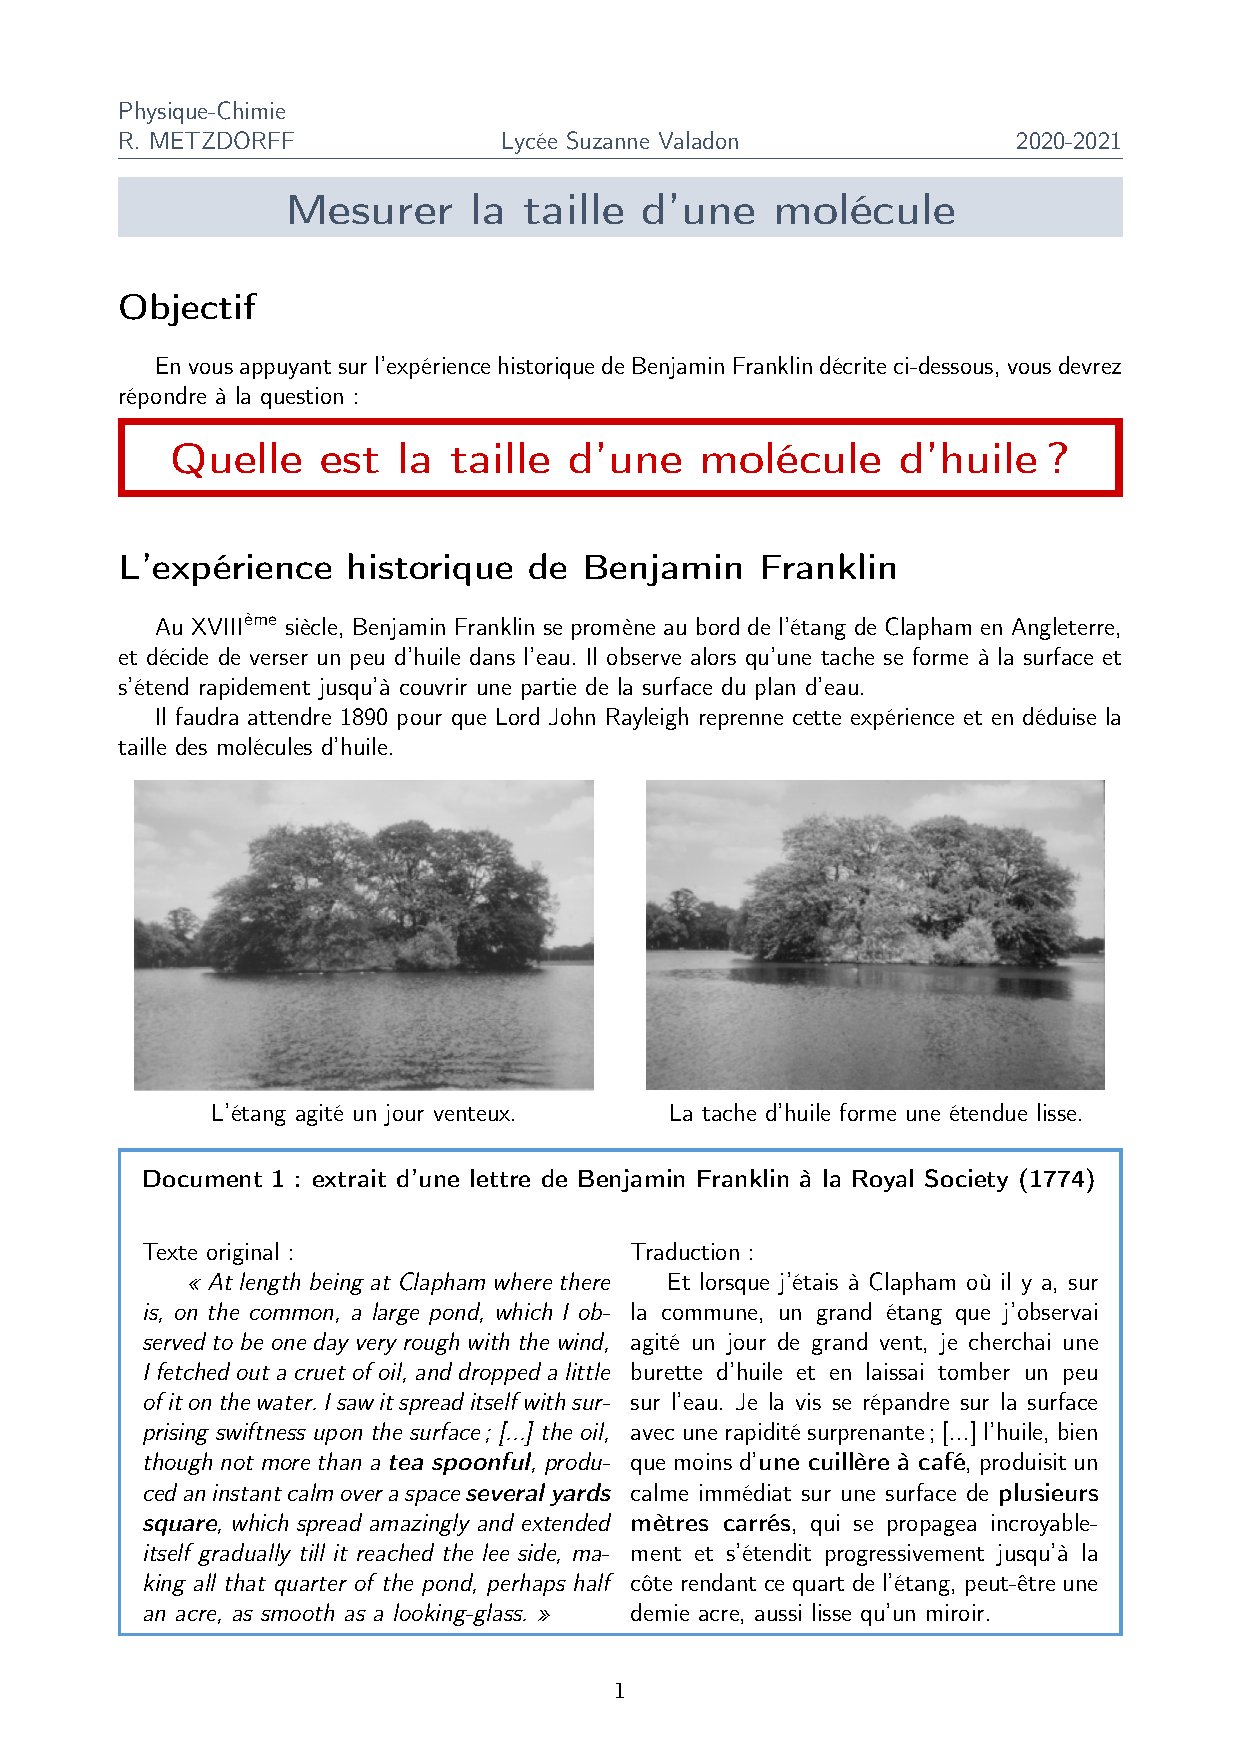
\includepdf[pages=-]{tp_franklin/tp_franklin_v3.pdf}

\end{document}

\begin{center}
\begin{tabular}{l|l}
\textbf{Compétences} & Aptitudes à vérifier \hfill \textbf{Suis-je capable de ... ?} \\
\hline
\hline
\app				 		& Me servir correctement des ressources disponibles (doc, énoncé, ...) \\
		         			& Choisir les informations qui me seront utiles \\
\hline
\anarai		  		& Faire une hypothèse, la justifier \\
							& \textbf{Élaborer un protocole qui répond à la question} \\
      						& Donner des conclusions à l'activité \\
\hline
\rea     				& \textbf{Faire des observations utiles à l'activité} \\
							& Réaliser correctement les calculs analytiques et/ou numériques \\
\hline
\val		      			& Dire si mes résultats sont en accord avec ceux attendus \\
			       			& \textbf{Avoir un regard critique sur mes résultats} \\
\hline
\com				  	& Rendre compte de façon écrite ou orale \\
		         			& Utiliser un vocabulaire et des modes de représentation adaptés \\
\hline
\rco         			& Restituer ses connaissances \\
\end{tabular}
\end{center}

\includepdf[pages=3-11]{../../../biblio/articles/rstl.1774.0044.pdf}
\includepdf[pages=-]{../../../biblio/articles/rspl.1889.0099.pdf}
\includepdf[pages=-]{../../../biblio/articles/pockels_surface_tension.pdf}
\includepdf[pages=2-]{../../../biblio/articles/ajp-jphysrad_1931_2_8_237_0.pdf}
\includepdf[pages=-]{../../../biblio/articles/17_JACS_Langmuir.pdf}
%\includepdf[pages=-]{../../../biblio/articles/}